\documentclass[border=5pt]{standalone}
\usepackage[utf8]{inputenc}
\usepackage[T1]{fontenc}
\usepackage{tikz}
\usetikzlibrary{shapes.geometric,arrows.meta,positioning,calc}

\definecolor{eegcolor}{RGB}{66,133,244}

\begin{document}
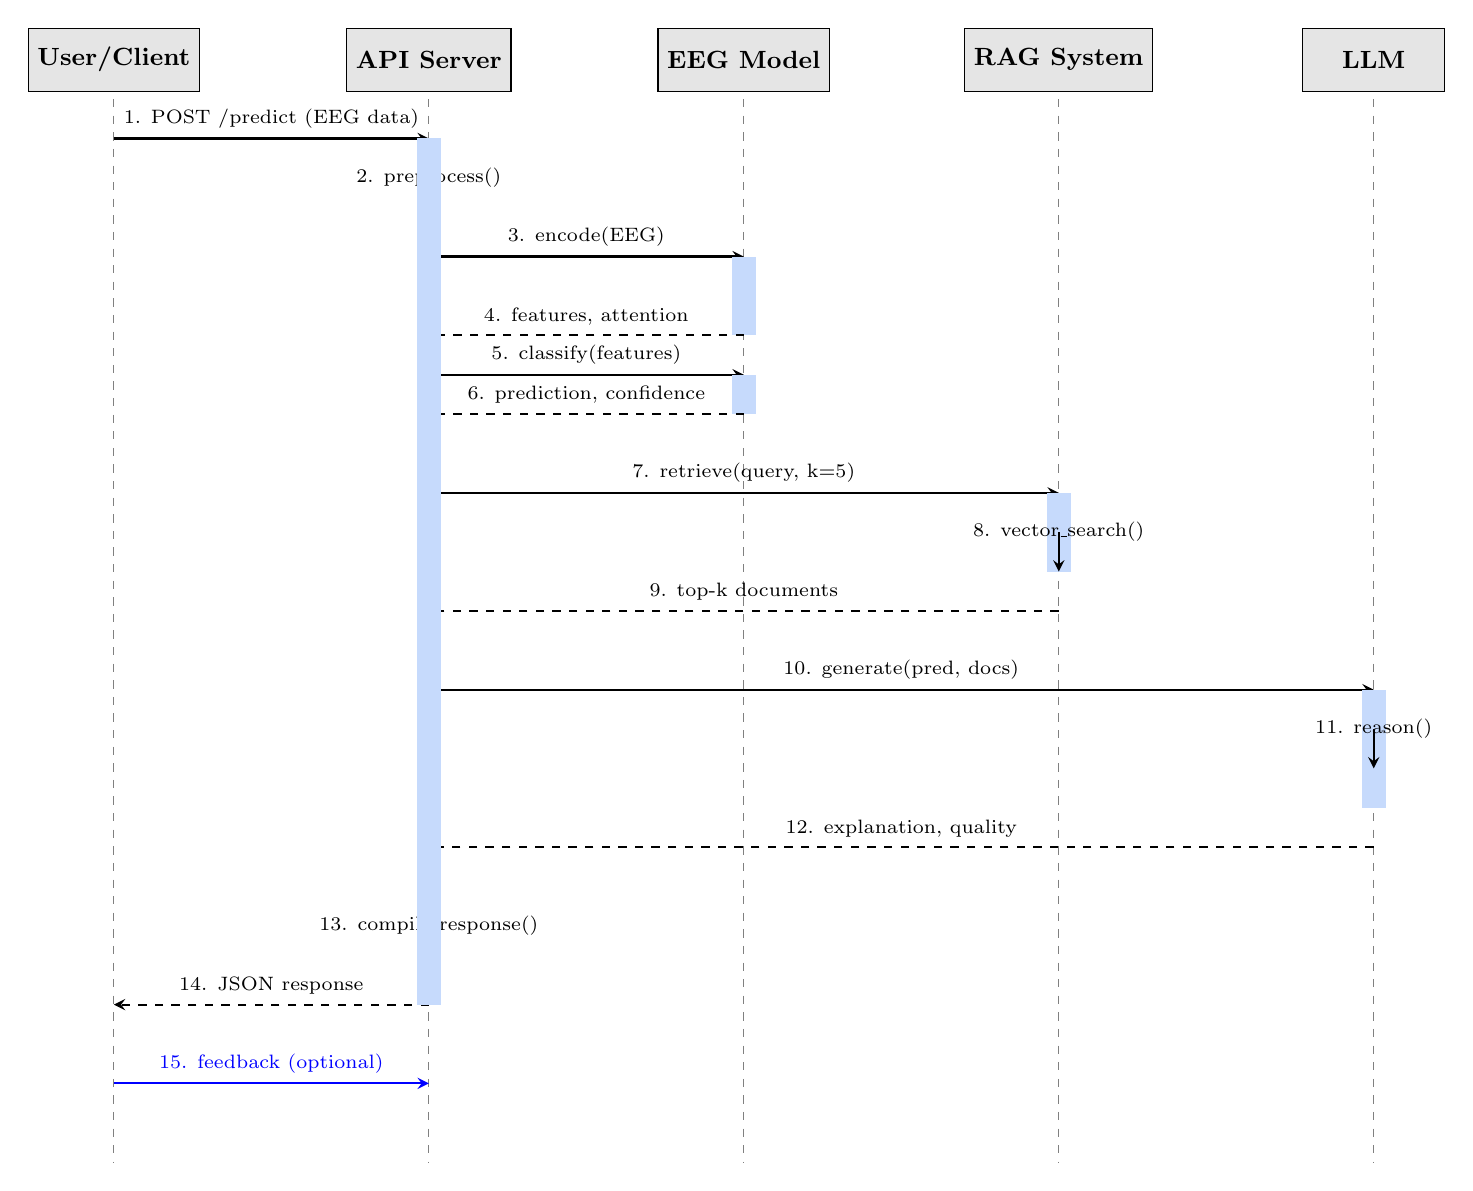
\begin{tikzpicture}[
    font=\small,
    actor/.style={rectangle, draw, fill=gray!20, minimum width=1.8cm, minimum height=0.8cm, font=\small\bfseries},
    lifeline/.style={dashed, gray},
    message/.style={->,>=stealth, thick},
    return/.style={->,>=stealth, thick, dashed},
    activation/.style={rectangle, fill=eegcolor!30, minimum width=0.3cm}
]

% Actors
\node[actor] (user) at (0,0) {User/Client};
\node[actor] (api) at (4,0) {API Server};
\node[actor] (model) at (8,0) {EEG Model};
\node[actor] (rag) at (12,0) {RAG System};
\node[actor] (llm) at (16,0) {LLM};

% Lifelines
\foreach \x in {0,4,8,12,16} {
    \draw[lifeline] (\x,-0.5) -- (\x,-14);
}

% Sequence numbers and messages
% 1. User sends EEG data
\draw[message] (0,-1) -- node[above, font=\scriptsize] {1. POST /predict (EEG data)} (4,-1);
\node[activation, minimum height=0.5cm] at (4,-1.25) {};

% 2. API preprocesses
\draw[message] (4,-1.5) -- node[above, font=\scriptsize] {2. preprocess()} (4,-2);

% 3. API sends to model
\draw[message] (4,-2.5) -- node[above, font=\scriptsize] {3. encode(EEG)} (8,-2.5);
\node[activation, minimum height=1cm] at (8,-3) {};

% 4. Model returns features
\draw[return] (8,-3.5) -- node[above, font=\scriptsize] {4. features, attention} (4,-3.5);

% 5. API requests prediction
\draw[message] (4,-4) -- node[above, font=\scriptsize] {5. classify(features)} (8,-4);
\node[activation, minimum height=0.5cm] at (8,-4.25) {};

% 6. Model returns prediction
\draw[return] (8,-4.5) -- node[above, font=\scriptsize] {6. prediction, confidence} (4,-4.5);

% 7. API queries RAG
\draw[message] (4,-5.5) -- node[above, font=\scriptsize] {7. retrieve(query, k=5)} (12,-5.5);
\node[activation, minimum height=1cm] at (12,-6) {};

% 8. RAG searches vector DB
\draw[message] (12,-6) -- node[above, font=\scriptsize] {8. vector\_search()} (12,-6.5);

% 9. RAG returns documents
\draw[return] (12,-7) -- node[above, font=\scriptsize] {9. top-k documents} (4,-7);

% 10. API sends to LLM
\draw[message] (4,-8) -- node[above, font=\scriptsize] {10. generate(pred, docs)} (16,-8);
\node[activation, minimum height=1.5cm] at (16,-8.75) {};

% 11. LLM processes
\draw[message] (16,-8.5) -- node[above, font=\scriptsize] {11. reason()} (16,-9);

% 12. LLM returns explanation
\draw[return] (16,-10) -- node[above, font=\scriptsize] {12. explanation, quality} (4,-10);

% 13. API compiles response
\draw[message] (4,-11) -- node[above, font=\scriptsize] {13. compile\_response()} (4,-11.5);

% 14. API returns to user
\draw[return] (4,-12) -- node[above, font=\scriptsize] {14. JSON response} (0,-12);

% 15. User feedback (optional)
\draw[message, blue] (0,-13) -- node[above, font=\scriptsize, blue] {15. feedback (optional)} (4,-13);

% Activation boxes
\node[activation, minimum height=11cm] at (4,-6.5) {};

\end{tikzpicture}
\end{document}
